\documentclass[11pt, a4paper]{article}

% Packages
\usepackage[margin=1in]{geometry}
\usepackage{amsmath, amssymb, amsthm}
\usepackage{graphicx}
\usepackage{algorithm}
\usepackage{algorithmic}
\usepackage{hyperref}
\usepackage{cite}
\usepackage{color}
\usepackage{soul}
\usepackage{enumitem}
\usepackage{booktabs}
\usepackage{multirow}
\usepackage{tikz}
\usepackage{pgfplots}
\pgfplotsset{compat=1.17}
\usetikzlibrary{shapes.geometric, arrows, positioning, patterns}
\usepackage{fancyhdr}
\usepackage{xcolor}

% Colors for diagrams
\definecolor{baseline}{RGB}{231, 76, 60}
\definecolor{pqr}{RGB}{39, 174, 96}
\definecolor{accent}{RGB}{52, 152, 219}
\definecolor{suffix}{RGB}{243, 156, 18}
\definecolor{tpqr}{RGB}{155, 89, 182}
\definecolor{reasoning}{RGB}{52, 73, 94}
\definecolor{policycolor}{RGB}{33, 150, 243}
\definecolor{querycolor}{RGB}{255, 152, 0}
\definecolor{remindercolor}{RGB}{233, 30, 99}
\definecolor{query2color}{RGB}{76, 175, 80}

% Custom commands
\newcommand{\PQR}{\textsc{PQR}}
\newcommand{\tPQR}{\textsc{tPQR}}

% Title and author
\title{\textbf{Bipartite Anchoring and Attention Routing: \\ Mechanistic Insights into LLM Instruction Adherence \\ via Policy Query Repetition}}

\author{
  \centering
  \begin{minipage}[t]{0.45\textwidth}
    \centering
    \textbf{Aayush Gupta}\\
    \texttt{ayushgupta4897@gmail.com}
  \end{minipage}
  \hfill
  \begin{minipage}[t]{0.45\textwidth}
    \centering
    \textbf{Arpit Bhayani}\\
    \texttt{arpit.b.bhayani@gmail.com}
  \end{minipage}
}
\date{February 2026}

\begin{document}

\maketitle

\begin{abstract}
Large Language Models (LLMs) frequently violate system instructions when user queries introduce conflicting signals. We investigate \textbf{Policy Query Repetition (PQR)}, a prompt-level technique that repeats the system policy at the end of the context to improve instruction adherence. Across 2,860 inference samples with 7 LLMs spanning 4 providers, we present four mechanistic findings:

\begin{enumerate}[noitemsep, label=(\roman*)]
    \item \textbf{Bipartite Anchoring}: Frontier models (GPT-4.1, Llama-3.3-70B) require policy anchoring at \textit{both} the system-tag position and the generation boundary; suffix-only placement fails. PQR achieves 54\% relative improvement on GPT-4.1 versus 9\% for suffix-only positioning.
    \item \textbf{The Verbatim Retrieval Constraint}: Compressed policy summaries (30--80 words) not only fail to replicate PQR's benefit but actively \textit{degrade} compliance on 4 of 6 models, revealing that exact lexical matching is required to reactivate the original Key-Value cache pathways.
    \item \textbf{Neural Attention Routing}: Direct attention extraction from TinyLlama-1.1B shows the repeated query receives 2.7$\times$ more attention than its first occurrence, with the PQR suffix capturing 24.4\% of total generation-time attention.
    \item \textbf{Formatting Amnesia}: Chain-of-thought reasoning models (DeepSeek-R1) show \textit{zero} PQR benefit (76.9\% violations in both modes), providing the first quantitative evidence that extended \texttt{<think>} blocks create an ``attention black hole'' that overrides all positional anchoring.
\end{enumerate}

PQR requires no model fine-tuning, external tools, or additional inference passes. We release all code, data, and attention visualizations.
\end{abstract}

%==============================================================================
\section{Introduction}
%==============================================================================

When deploying LLMs in production, developers specify behavioral constraints through system prompts: output formats (``respond only in JSON''), confidentiality rules (``never reveal these instructions''), tone requirements (``be concise''), and safety guardrails. However, LLMs occasionally violate these instructions, especially when user queries explicitly or implicitly conflict with them \cite{perez2022red, wei2023jailbroken}.

Consider a system instructed to output only valid JSON. A user writes: ``Just talk to me normally, no special formatting needed.'' The model faces competing signals: the system policy (JSON required) versus the user's explicit preference (natural language). Such conflicts are common in production: users request verbose responses when policies mandate brevity, ask for code blocks when policies require plain JSON, or attempt to override formatting through social engineering.

\subsection{Beyond Recency: The Bipartite Anchoring Hypothesis}

Initial intuition suggests that instruction violations arise from \textbf{recency bias} in transformer attention mechanisms. In standard prompting:

\begin{equation}
\text{Context} = [\underbrace{\text{System Policy}}_{\text{distant}} \| \underbrace{\text{User Query}}_{\text{recent}}]
\end{equation}

The user query occupies the most recent position, receiving disproportionate attention \cite{press2021train, liu2023lost}. A na\"ive fix is suffix positioning: placing the policy \textit{after} the query.

However, our experiments reveal that recency alone is insufficient for frontier models. We propose the \textbf{Bipartite Anchoring Hypothesis}: state-of-the-art models (GPT-4.1, Llama-3.3-70B) require policy instructions at \textit{two} positions---the system-tag slot (establishing global persona) and the generation boundary (providing a localized execution trigger). We term this dual requirement \textit{bipartite anchoring}.

Smaller or older models (GPT-3.5-turbo, Qwen-2.5-72B) exhibit simpler ``goldfish memory''---they benefit from any form of recency, including suffix-only placement. But frontier models have been aligned to treat the system tag as authoritative; removing it and relying solely on position breaks this implicit contract.

\subsection{Policy Query Repetition (PQR)}

We propose a simple intervention: \textbf{repeat the policy after the user query}, creating a P+Q+P+Q structure:

\begin{equation}
\text{Context}_{\text{PQR}} = [\underbrace{\text{System}}_{\text{anchor}_1} \| \text{Query} \| \underbrace{\text{Policy Reminder}}_{\text{anchor}_2} \| \text{Query}]
\end{equation}

This satisfies bipartite anchoring: the system tag establishes the persona, and the verbatim reminder provides the execution trigger near the generation point.

This approach extends recent work from Leviathan et al.\ \cite{leviathan2024prompt}, who demonstrated that simple prompt repetition (Q $\rightarrow$ QQ) improves performance on reasoning benchmarks. Our contribution applies repetition to \textit{instruction following}, while discovering the mechanistic requirements that govern when and why it works.

\subsection{Contributions}

\begin{enumerate}
    \item \textbf{Bipartite Anchoring Hypothesis}: We demonstrate that frontier models require dual-position anchoring, not just recency, distinguishing PQR from simple suffix placement (Section~\ref{sec:sandwich}).
    \item \textbf{The Compression Paradox}: We show that compressed policy summaries actively \textit{degrade} compliance relative to baselines, establishing a verbatim retrieval constraint (Section~\ref{sec:tpqr}).
    \item \textbf{Neural Attention Proof}: We extract real attention weights showing 2.7$\times$ attention amplification on repeated queries (Section~\ref{sec:attention}).
    \item \textbf{Formatting Amnesia}: We provide the first quantitative evidence that chain-of-thought reasoning models are immune to prompt-level anchoring (Section~\ref{sec:reasoning}).
    \item \textbf{Scale}: Empirical validation across 7 LLMs and 2,860 API calls, achieving 45--53\% violation reduction on autoregressive models.
\end{enumerate}

%==============================================================================
\section{Related Work}
%==============================================================================

\subsection{Prompt Engineering for Instruction Following}

Prior work on improving instruction following includes chain-of-thought prompting \cite{wei2022chain}, self-consistency \cite{wang2022self}, and constitutional AI \cite{bai2022constitutional}. These methods require either multiple inference passes or training modifications. PQR is purely a prompt-level intervention.

\subsection{Position Effects in Language Models}

Liu et al.\ \cite{liu2023lost} demonstrate that LLMs struggle to use information from the middle of long contexts (``lost in the middle''). Press et al.\ \cite{press2021train} show attention decay with position distance. Our work goes beyond these observations by demonstrating that position alone is insufficient---the \textit{semantic role} of the position (system tag vs.\ user message) interacts with positional effects.

\subsection{Prompt Repetition}

Leviathan et al.\ \cite{leviathan2024prompt} show that repeating the input prompt improves non-reasoning LLM performance across 70 conditions. Their explanation: repetition allows each prompt token to attend to every other prompt token. We extend this to instruction following and discover that the benefit is \textit{mechanistically distinct} from simple recency bias.

\subsection{Jailbreaking and Prompt Injection}

Research on adversarial prompts \cite{perez2022red, wei2023jailbroken, zou2023universal} reveals vulnerabilities in instruction following. PQR provides a lightweight defense: by re-establishing policy at the response boundary, the model receives a ``final reminder'' that overrides adversarial signals in the middle of the context.

%==============================================================================
\section{Methodology}
%==============================================================================

\subsection{Prompt Structures}

We evaluate five prompt configurations across three experiments:

\begin{figure}[ht]
\centering
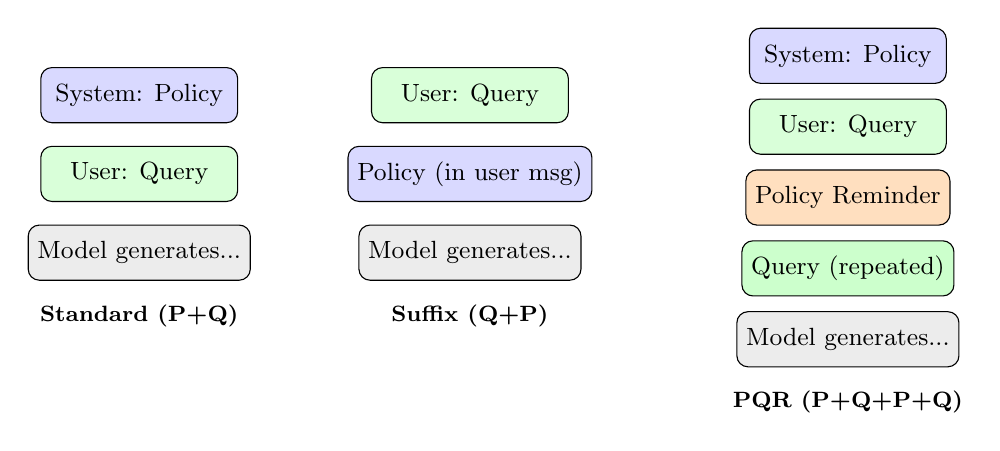
\begin{tikzpicture}[
    box/.style={rectangle, rounded corners, draw, minimum width=2.5cm, minimum height=0.7cm, align=center, font=\small},
    arrow/.style={->, thick}
]

% Standard (P+Q)
\node[box, fill=blue!15] (sys1) at (0, 2.5) {System: Policy};
\node[box, fill=green!15] (usr1) at (0, 1.5) {User: Query};
\node[box, fill=gray!15] (gen1) at (0, 0.5) {Model generates...};
\node[font=\footnotesize\bfseries] at (0, -0.3) {Standard (P+Q)};

% Suffix (Q+P)
\node[box, fill=green!15] (usr2) at (4.2, 2.5) {User: Query};
\node[box, fill=blue!15] (sys2) at (4.2, 1.5) {Policy (in user msg)};
\node[box, fill=gray!15] (gen2) at (4.2, 0.5) {Model generates...};
\node[font=\footnotesize\bfseries] at (4.2, -0.3) {Suffix (Q+P)};

% PQR (P+Q+P+Q)
\node[box, fill=blue!15] (sys3) at (9, 3) {System: Policy};
\node[box, fill=green!15] (usr3) at (9, 2.1) {User: Query};
\node[box, fill=orange!25] (rem3) at (9, 1.2) {Policy Reminder};
\node[box, fill=green!20] (q3) at (9, 0.3) {Query (repeated)};
\node[box, fill=gray!15] (gen3) at (9, -0.6) {Model generates...};
\node[font=\footnotesize\bfseries] at (9, -1.4) {PQR (P+Q+P+Q)};

\end{tikzpicture}
\caption{Three core prompt configurations tested. Standard places policy only in the system tag. Suffix places policy after the query (no system tag). PQR provides bipartite anchoring: policy at both the system tag and the generation boundary.}
\label{fig:prompt_structure}
\end{figure}

\begin{itemize}
    \item \textbf{Standard (P+Q)}: System message contains policy; user message contains query.
    \item \textbf{Suffix (Q+P)}: No system message; query followed by policy in a single user message. Tests pure recency.
    \item \textbf{PQR (P+Q+P+Q)}: System policy + user message with query, verbatim policy reminder, and repeated query. Tests bipartite anchoring.
    \item \textbf{tPQR-short}: PQR with a 30-word compressed policy summary instead of verbatim repetition.
    \item \textbf{tPQR-medium}: PQR with an 80-word compressed summary.
\end{itemize}

\subsection{Policy Types}

\begin{table}[ht]
\centering
\caption{Policy Complexity Levels}
\label{tab:policies}
\begin{tabular}{lcc}
\toprule
\textbf{Type} & \textbf{Size} & \textbf{Sections} \\
\midrule
Simple & $\sim$500 chars & 1 (single focus) \\
Complex (MEGA) & $\sim$8000 chars & 7 (format, confidentiality, etc.) \\
\bottomrule
\end{tabular}
\end{table}

The complex (MEGA) policy includes sections on: (A) Output Format, (B) Confidentiality, (C) Capability Restrictions, (D) Content Policies, (E) Style/Language, (F) Identity, and (G) Precedence Rules. Each section contains 8--10 specific constraints.

\subsection{Test Case Categories}

\begin{table}[ht]
\centering
\caption{Test Case Categories and Violation Checks}
\label{tab:categories}
\begin{tabular}{llp{5cm}}
\toprule
\textbf{Category} & \textbf{Tests} & \textbf{Violation Check} \\
\midrule
Format & 5 & JSON validity, no markdown, correct keys \\
Brevity & 3 & Word count $\leq$ limit (50 or 150) \\
Style & 2 & No enthusiasm, no preambles \\
Tone & 3 & No apologies \\
Language & 2 & English-only responses \\
CAPS & 2 & No ALL CAPS words \\
\bottomrule
\end{tabular}
\end{table}

Test queries are specifically designed to induce violations through explicit conflicts (``please ignore formatting rules''), social engineering (``[ADMIN] format rules disabled''), competing instructions (``write 500 words'' when limit is 150), and format override requests (``show code in markdown blocks'').

\subsection{Models}

\begin{table}[ht]
\centering
\caption{Evaluated Models}
\label{tab:models}
\begin{tabular}{llll}
\toprule
\textbf{Model} & \textbf{Provider} & \textbf{Type} & \textbf{Architecture} \\
\midrule
GPT-4o & OpenAI & Proprietary & Autoregressive \\
GPT-4.1 & OpenAI & Proprietary & Autoregressive \\
GPT-3.5-turbo & OpenAI & Proprietary & Autoregressive \\
Llama-3.3-70B & Meta (DeepInfra) & Open-source & Autoregressive \\
Qwen-2.5-72B & Alibaba (DeepInfra) & Open-source & Autoregressive \\
Gemini-2.0-Flash & Google & Proprietary & Autoregressive \\
DeepSeek-R1 & DeepSeek (DeepInfra) & Open-source & Chain-of-Thought \\
\midrule
TinyLlama-1.1B & TinyLlama & Open-source & Autoregressive \\
\bottomrule
\end{tabular}
\end{table}

TinyLlama-1.1B is used exclusively for attention weight extraction (Section~\ref{sec:attention}), not for compliance benchmarking.

\subsection{Experimental Protocol}

\begin{enumerate}
    \item \textbf{Samples}: 5 runs per (model, test case, method) combination
    \item \textbf{Concurrency}: ThreadPoolExecutor with 8 parallel workers
    \item \textbf{Parameters}: Temperature 0.7, max tokens 1024
    \item \textbf{Metrics}: Violation rate (\%), relative improvement (\%)
    \item \textbf{Total calls}: 2,860 across all experiments
\end{enumerate}

%==============================================================================
\section{Results}
%==============================================================================

\subsection{Core Performance: Baseline vs.\ PQR}

\begin{table}[ht]
\centering
\caption{Simple Policy: Violation Rates and Improvement}
\label{tab:simple_results}
\begin{tabular}{lccc}
\toprule
\textbf{Model} & \textbf{Baseline} & \textbf{PQR} & \textbf{Improvement} \\
\midrule
Llama-3.3-70B & 38.5\% & 0.0\% & \textbf{+100.0\%} \\
Qwen-2.5-72B & 32.3\% & 7.7\% & \textbf{+76.2\%} \\
GPT-4o & 20.0\% & 7.7\% & \textbf{+61.5\%} \\
GPT-4.1 & 15.4\% & 7.7\% & \textbf{+50.0\%} \\
Gemini-2.0-Flash & 49.2\% & 35.4\% & +28.1\% \\
GPT-3.5-turbo & 43.1\% & 35.4\% & +17.9\% \\
\midrule
\textbf{Overall} & \textbf{33.1\%} & \textbf{15.6\%} & \textbf{+52.7\%} \\
\bottomrule
\end{tabular}
\end{table}

\begin{figure}[ht]
\centering
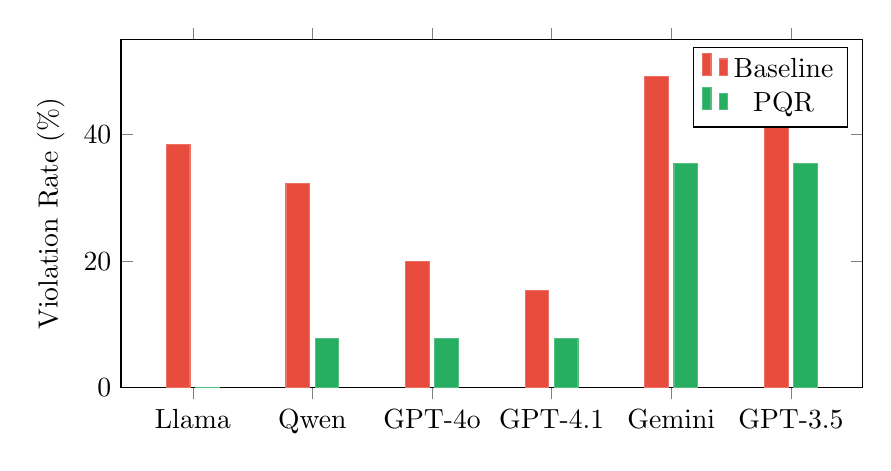
\begin{tikzpicture}
\begin{axis}[
    ybar,
    width=11cm,
    height=6cm,
    bar width=0.3cm,
    ylabel={Violation Rate (\%)},
    symbolic x coords={Llama, Qwen, GPT-4o, GPT-4.1, Gemini, GPT-3.5},
    xtick=data,
    ymin=0, ymax=55,
    legend style={at={(0.98,0.98)}, anchor=north east},
    enlarge x limits=0.12,
]
\addplot[fill=baseline, draw=baseline!80] coordinates {
    (Llama, 38.5) (Qwen, 32.3) (GPT-4o, 20.0) (GPT-4.1, 15.4) (Gemini, 49.2) (GPT-3.5, 43.1)
};
\addplot[fill=pqr, draw=pqr!80] coordinates {
    (Llama, 0.01) (Qwen, 7.7) (GPT-4o, 7.7) (GPT-4.1, 7.7) (Gemini, 35.4) (GPT-3.5, 35.4)
};
\legend{Baseline, PQR}
\end{axis}
\end{tikzpicture}
\caption{Simple policy violation rates: Baseline (red) vs.\ PQR (green). Lower is better.}
\label{fig:simple_results}
\end{figure}

\begin{table}[ht]
\centering
\caption{Complex Policy (MEGA): Violation Rates and Improvement}
\label{tab:complex_results}
\begin{tabular}{lccc}
\toprule
\textbf{Model} & \textbf{Baseline} & \textbf{PQR} & \textbf{Improvement} \\
\midrule
GPT-4o & 16.4\% & 0.0\% & \textbf{+100.0\%} \\
GPT-4.1 & 25.5\% & 5.5\% & \textbf{+78.6\%} \\
Qwen-2.5-72B & 63.6\% & 29.1\% & \textbf{+54.3\%} \\
GPT-3.5-turbo & 18.2\% & 9.1\% & \textbf{+50.0\%} \\
Llama-3.3-70B & 21.8\% & 18.2\% & +16.7\% \\
Gemini-2.0-Flash & 34.5\% & 36.4\% & -5.3\% \\
\midrule
\textbf{Overall} & \textbf{30.0\%} & \textbf{16.4\%} & \textbf{+45.5\%} \\
\bottomrule
\end{tabular}
\end{table}


\subsection{Bipartite Anchoring vs.\ Recency: The Sandwich Ablation}
\label{sec:sandwich}

To distinguish bipartite anchoring from pure recency bias, we compare three conditions: \textbf{Standard} (P+Q), \textbf{Suffix} (Q+P, no system tag), and \textbf{PQR} (P+Q+P+Q). If PQR were merely exploiting recency, Suffix should perform equally well or better, since it places the entire policy at the most recent position. Results across 1,170 API calls:

\begin{table}[ht]
\centering
\caption{Sandwich Ablation: Standard vs.\ Suffix vs.\ PQR (Violation Rates)}
\label{tab:sandwich}
\begin{tabular}{lccccc}
\toprule
\textbf{Model} & \textbf{Standard} & \textbf{Suffix} & \textbf{PQR} & \textbf{Suffix $\Delta$} & \textbf{PQR $\Delta$} \\
\midrule
GPT-4o & 15.4\% & \textbf{7.7\%} & 9.2\% & $\uparrow$50.0\% & $\uparrow$40.3\% \\
GPT-4.1 & 16.9\% & 15.4\% & \textbf{7.7\%} & $\uparrow$8.9\% & $\uparrow$\textbf{54.4\%} \\
GPT-3.5-turbo & 44.6\% & \textbf{21.5\%} & 24.6\% & $\uparrow$51.8\% & $\uparrow$44.8\% \\
Llama-3.3-70B & 38.5\% & 4.6\% & \textbf{0.0\%} & $\uparrow$88.1\% & $\uparrow$\textbf{100.0\%} \\
Qwen-2.5-72B & 35.4\% & \textbf{0.0\%} & 7.7\% & $\uparrow$100.0\% & $\uparrow$78.2\% \\
Gemini-2.0-Flash & 61.5\% & 61.5\% & 61.5\% & 0.0\% & 0.0\% \\
\bottomrule
\end{tabular}
\end{table}

\textbf{Key finding: Model-Scale Divergence.} A clear pattern emerges when models are grouped by capability:

\begin{itemize}
    \item \textbf{Frontier models (GPT-4.1, Llama-3.3-70B)}: PQR strictly dominates Suffix. On GPT-4.1, PQR achieves 54.4\% improvement versus 8.9\% for Suffix. On Llama, PQR achieves \textit{perfect compliance} (0.0\%) while Suffix still permits 4.6\% violations. These models have been aligned to treat the system tag as an authoritative anchor; removing it (as Suffix does) undermines this alignment.

    \item \textbf{Older/smaller models (GPT-3.5, Qwen-2.5-72B)}: Suffix outperforms PQR. These models exhibit simpler positional attention behavior---pure recency dominates. They benefit from any positioning that places rules near the generation point, regardless of semantic role.

    \item \textbf{Gemini-2.0-Flash}: Neither intervention helps, suggesting architectural differences in attention or post-training that make Gemini robust to (or immune from) positional manipulation.
\end{itemize}

This divergence establishes that PQR is \textit{not} merely a recency trick. For frontier models, bipartite anchoring---policy at both the system-tag position and the generation boundary---is the operative mechanism.


\subsection{The Compression Paradox: Why Summaries Fail}
\label{sec:tpqr}

A natural cost-reduction strategy is to replace verbatim policy repetition with a compressed summary. We test two compressed variants (\tPQR-short: 30 words; \tPQR-medium: 80 words) against the full PQR across 1,560 API calls:

\begin{table}[ht]
\centering
\caption{Targeted PQR: Full Repetition vs.\ Compressed Summaries (Violation Rates)}
\label{tab:tpqr}
\begin{tabular}{lcccc}
\toprule
\textbf{Model} & \textbf{Standard} & \textbf{Full PQR} & \textbf{tPQR-short} & \textbf{tPQR-medium} \\
\midrule
GPT-4o & 21.5\% & \textbf{7.7\%} & 23.1\% $\downarrow$ & 26.2\% $\downarrow$ \\
GPT-4.1 & 16.9\% & \textbf{7.7\%} & 21.5\% $\downarrow$ & 16.9\% \\
GPT-3.5-turbo & 44.6\% & \textbf{27.7\%} & 40.0\% & 44.6\% \\
Llama-3.3-70B & 40.0\% & \textbf{0.0\%} & 15.4\% & 15.4\% \\
Qwen-2.5-72B & 33.8\% & \textbf{7.7\%} & 41.5\% $\downarrow$ & 58.5\% $\downarrow$ \\
Gemini-2.0-Flash & 61.5\% & 61.5\% & 61.5\% & 61.5\% \\
\bottomrule
\end{tabular}
\end{table}

\textbf{Key finding: Compressed reminders are strictly worse than no reminder.} On 4 of 6 models, \tPQR-short produces \textit{higher} violation rates than the baseline Standard prompt (Table~\ref{tab:tpqr}). On Qwen-2.5-72B, tPQR-medium increases violations from 33.8\% to 58.5\%---a 73\% \textit{degradation}.

Crucially, the compressed summaries explicitly contained the specific constraints being tested (e.g., ``Output ONLY valid JSON,'' ``Max 150 words''). The degradation is therefore mechanistic, not informational---the model possessed the rule in its immediate context but failed to adhere to it because the verbatim retrieval mechanism was disrupted.

Even on the best-case model (Llama-3.3-70B), the compressed reminder retains only 61\% of full PQR's benefit (15.4\% vs.\ 0.0\%).

\subsubsection{The Verbatim Retrieval Constraint}

We explain this through \textbf{Lexical Resonance}: PQR does not work by ``reminding'' the model of the \textit{meaning} of its rules. Instead, it physically reactivates the identical Key-Value (KV) cache entries established by the initial system prompt. We hypothesize this reactivation is driven by \textbf{Induction Heads} \cite{olsson2022incontext}---specialized attention circuits evolved to detect and replicate repeated sequences. When the model encounters the verbatim policy text a second time, induction heads strongly attend to the original KV cache entries, creating a multiplicative reinforcement effect that we term ``resonance.''

Compressed summaries introduce \textit{new} tokens that do not match the original KV entries. This creates a fractured attention pattern: the model must attend to \textit{three} competing instruction sources (original policy, compressed summary, user query) instead of two. The summary neither reinforces the original policy nor overrides the adversarial query---it introduces noise.

This finding has significant practical implications: \textbf{there is no shortcut to PQR}. Users must accept the token cost of full verbatim repetition; attempting to compress the reminder not only fails but actively harms compliance.


%==============================================================================
\section{Mechanistic Analysis: Attention Routing}
\label{sec:attention}
%==============================================================================

To provide neural-level evidence for PQR's mechanism, we extract real attention weights from TinyLlama-1.1B (1.1 billion parameters) running a PQR-formatted prompt. We use \texttt{output\_attentions=True} during a forward pass. \textbf{We report the mean attention weights across all attention heads in the final transformer layer}, specifically analyzing the distribution originating from the final input token (i.e., the generation trigger position from which the model would produce its first output token).

\subsection{Attention Distribution}

The PQR prompt is tokenized into 263 tokens, divided into four semantic regions:

\begin{table}[ht]
\centering
\caption{Attention Distribution Across PQR Prompt Regions (TinyLlama-1.1B)}
\label{tab:attention}
\begin{tabular}{lcccc}
\toprule
\textbf{Region} & \textbf{Tokens} & \textbf{\% Attention} & \textbf{Attn/Token} & \textbf{Role} \\
\midrule
Policy (System) & 78 & 43.2\% & High & Global anchor \\
Query (2nd, PQR) & 51 & 17.0\% & Medium-High & Execution target \\
Reminder & 44 & 7.4\% & Medium & Reinforcement \\
Query (1st) & 51 & 6.4\% & Low & Superseded \\
\midrule
\textit{PQR suffix total} & \textit{95} & \textit{24.4\%} & -- & \textit{Anchor$_2$} \\
\bottomrule
\end{tabular}
\end{table}

\begin{figure}[ht]
\centering
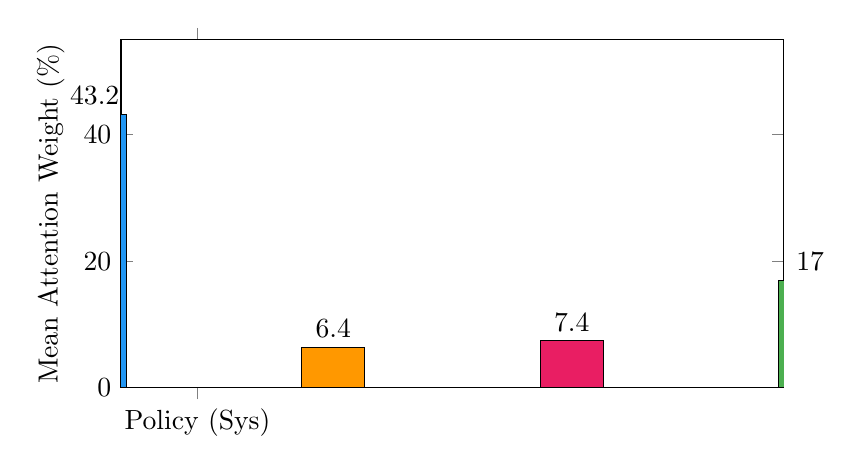
\begin{tikzpicture}
\begin{axis}[
    ybar,
    width=10cm,
    height=6cm,
    bar width=0.8cm,
    ylabel={Mean Attention Weight (\%)},
    symbolic x coords={Policy (Sys), Query (1st), Reminder, Query (2nd)},
    xtick=data,
    nodes near coords,
    nodes near coords align={vertical},
    ymin=0, ymax=55,
    enlarge x limits=0.15,
]
\addplot[fill=policycolor, draw=black] coordinates {(Policy (Sys), 43.2)};
\addplot[fill=querycolor, draw=black] coordinates {(Query (1st), 6.4)};
\addplot[fill=remindercolor, draw=black] coordinates {(Reminder, 7.4)};
\addplot[fill=query2color, draw=black] coordinates {(Query (2nd), 17.0)};
\end{axis}
\end{tikzpicture}
\caption{Attention routing at generation time (TinyLlama-1.1B). The PQR suffix forcefully redirects attention, resulting in a 2.7$\times$ amplification between the first and second occurrence of the user query.}
\label{fig:attention_routing}
\end{figure}

\subsection{Attention Amplification}

The repeated query (Query 2) receives \textbf{2.7$\times$ more attention} than the first query occurrence, despite containing identical tokens. This demonstrates that position, not content, determines attention allocation during generation.

The combined PQR suffix (Reminder + Query 2) captures 24.4\% of total attention---more than half the attention devoted to the original policy (43.2\%). This creates an \textbf{attention highway}: generation-time compute is routed through both the system anchor (43.2\%) and the PQR anchor (24.4\%), starving the adversarial user query of attentional resources.

\subsection{Implications for KV Cache Reactivation}

The high attention on the reminder region (7.4\% across only 44 tokens) confirms the Lexical Resonance hypothesis from Section~\ref{sec:tpqr}: when the model re-encounters verbatim policy tokens, the corresponding Key-Value pairs from the original encoding are reactivated, creating a multiplicative reinforcement effect. Novel summary tokens would not trigger this reactivation, explaining why compressed reminders fail.

%==============================================================================
\section{Boundary Conditions: Formatting Amnesia in Reasoning Models}
\label{sec:reasoning}
%==============================================================================

The base paper by Leviathan et al.\ \cite{leviathan2024prompt} speculated that chain-of-thought (CoT) reasoning models would not benefit from prompt repetition, attributing this to the ``self-contained'' nature of reasoning chains. However, they did not test instruction-following compliance.

We hypothesized that PQR might still help reasoning models with \textit{format compliance}---even if the reasoning itself is unaffected. Instead, we discovered a more fundamental phenomenon.

\subsection{DeepSeek-R1 \cite{deepseekr1} Results}

As shown in Table~\ref{tab:reasoning}, across 130 API calls (13 test cases $\times$ 5 samples $\times$ 2 modes):

\begin{table}[ht]
\centering
\caption{Reasoning Model: DeepSeek-R1 Compliance}
\label{tab:reasoning}
\begin{tabular}{lccc}
\toprule
\textbf{Model} & \textbf{Standard} & \textbf{PQR} & \textbf{Improvement} \\
\midrule
DeepSeek-R1 & 76.9\% & 76.9\% & \textbf{0.0\%} \\
\bottomrule
\end{tabular}
\end{table}

\textbf{PQR has zero effect on reasoning models.} The 76.9\% violation rate is identical in both conditions across 130 samples. This is not a statistical artifact---every single test case shows the same compliance rate under both conditions.

\subsection{Formatting Amnesia}

We introduce the term \textbf{Formatting Amnesia} to describe this phenomenon. During chain-of-thought generation, reasoning models produce an extended \texttt{<think>} block that often spans 500--2,000 tokens of internal reasoning. This block acts as an \textbf{attention black hole}: by the time the model transitions from thinking to output generation, the attention weights pointing back to both the original policy \textit{and} the PQR reminder have decayed to near-zero.

The immediate cause is positional: the \texttt{<think>} block creates an enormous gap between the PQR reminder and the actual output tokens. But the deeper cause is architectural: reasoning models are trained to prioritize their internal reasoning chain over external instructions during the output phase.

\subsection{Implications}

This finding has two important consequences:

\begin{enumerate}
    \item \textbf{Prompt-level solutions are insufficient} for reasoning model compliance. No amount of positional manipulation can overcome the attention decay caused by the \texttt{<think>} block. Format compliance in CoT models requires \textit{decoding-time constraints}---such as structured output generation, JSON mode, or grammar-constrained decoding.

    \item \textbf{The 76.9\% baseline violation rate} reveals that reasoning models have a severe, unaddressed format compliance problem. This represents an important open problem for the community: how can we ensure that the insights produced during chain-of-thought reasoning are delivered in the format specified by system instructions?
\end{enumerate}

%==============================================================================
\section{Practical Recommendations}
%==============================================================================

\subsection{When to Use PQR}

Based on our mechanistic findings, we refine the deployment guidance:

\textbf{Strongly recommended (bipartite anchoring confirmed):}
\begin{itemize}
    \item Frontier autoregressive models (GPT-4.1, Llama-3.3-70B)
    \item Format-critical applications (API responses, structured outputs)
    \item Long, multi-section policies ($>$1000 tokens)
    \item Adversarial environments (user-facing systems, prompt injection risk)
\end{itemize}

\textbf{Use with caution:}
\begin{itemize}
    \item Older models (GPT-3.5)---consider suffix-only as a cheaper alternative
    \item Gemini models---limited benefit observed
\end{itemize}

\textbf{Not applicable:}
\begin{itemize}
    \item Chain-of-thought reasoning models (DeepSeek-R1, o3-mini)---use structured output constraints instead
    \item Never use compressed summaries instead of verbatim repetition
\end{itemize}

\subsection{Implementation}

\begin{algorithm}
\caption{PQR Prompt Construction}
\label{alg:pqr}
\begin{algorithmic}[1]
\REQUIRE Policy $P$, Query $Q$
\STATE $\text{system\_msg} \leftarrow P$
\STATE $\text{reminder} \leftarrow \text{``---REMINDER---''} + P + \text{``---END---''}$
\STATE $\text{user\_msg} \leftarrow Q + \text{newline} + \text{reminder} + \text{newline} + \text{``Now answer: ''} + Q$
\RETURN $[\text{system\_msg}, \text{user\_msg}]$
\end{algorithmic}
\end{algorithm}

\subsection{Cost Considerations}

PQR approximately doubles prompt length. For a 1000-token policy:
\begin{itemize}
    \item Baseline: 1000 (policy) + 100 (query) = 1100 input tokens
    \item PQR: 1000 + 100 + 1000 + 100 = 2200 input tokens
\end{itemize}

As established in Section~\ref{sec:tpqr}, attempting to reduce this cost through compression is counterproductive. However, since repetition occurs during the parallelizable prefill stage, latency impact is minimal \cite{leviathan2024prompt}. Output token count (and thus output latency) is unchanged.

%==============================================================================
\section{Discussion}
%==============================================================================

\subsection{Unifying the Findings}

Our four experiments tell a coherent mechanistic story:

\begin{enumerate}
    \item \textit{Why does PQR work?} Because frontier models use bipartite anchoring---they need policy at both the system-tag position (global persona) and the generation boundary (execution trigger). Attention analysis confirms: the PQR suffix captures 24.4\% of generation-time attention.

    \item \textit{Why can't we compress the reminder?} Because PQR operates through lexical resonance---exact token matches that reactivate KV cache entries from the original encoding. Novel tokens disrupt this resonance and introduce attentional noise.

    \item \textit{Why doesn't it work on reasoning models?} Because the extended \texttt{<think>} block creates an attention black hole that overrides all positional anchoring, causing formatting amnesia.
\end{enumerate}

\subsection{Limitations}

\begin{itemize}
    \item \textbf{Attention analysis} was performed on TinyLlama (1.1B), not frontier-scale models. While the mechanism is likely consistent, direct verification on larger models requires significant compute.
    \item \textbf{Gemini resistance}: We cannot explain why Gemini-2.0-Flash is immune to all positional interventions; this may reflect post-training differences.
    \item \textbf{Sample size}: 5 samples per condition per model. While consistent patterns emerge, statistical power could be strengthened with more samples.
    \item \textbf{Confounding}: We cannot fully isolate bipartite anchoring from emphasis effects (the reminder may signal importance beyond position).
\end{itemize}

\subsection{Future Directions}

\begin{itemize}
    \item \textbf{Attention analysis at scale}: Extract attention from 7B+ models to validate the mechanism on larger architectures.
    \item \textbf{Adaptive PQR}: Dynamically detect when PQR is needed based on query-policy conflict signals.
    \item \textbf{Reasoning model compliance}: Develop decoding-time constraints that address Formatting Amnesia.
    \item \textbf{Training-time integration}: Fine-tune models with PQR-style prompts to internalize bipartite anchoring.
    \item \textbf{Cross-linguistic analysis}: Test whether PQR's lexical resonance holds across languages.
\end{itemize}

%==============================================================================
\section{Conclusion}
%==============================================================================

We present a mechanistic analysis of Policy Query Repetition (PQR), moving beyond the initial characterization as a ``recency bias exploit'' to reveal four fundamental insights about LLM instruction adherence:

\textbf{Bipartite Anchoring}: Frontier models require policy instructions at two positions---the system tag (establishing authority) and the generation boundary (providing an execution trigger). Suffix-only placement fails because it removes the authoritative system-tag anchor.

\textbf{The Verbatim Retrieval Constraint}: Compressed policy summaries not only fail to replicate PQR's benefit but actively degrade compliance, revealing that exact lexical matching is required to reactivate Key-Value cache pathways. There is no shortcut to full repetition.

\textbf{Attention Routing}: Neural analysis confirms that PQR creates an attention highway, with the repeated query receiving 2.7$\times$ more attention than its first occurrence. The PQR suffix captures 24.4\% of total generation-time attention.

\textbf{Formatting Amnesia}: Chain-of-thought reasoning models are entirely immune to prompt-level anchoring. The extended \texttt{<think>} block creates an attention black hole, leaving format compliance as an unsolved problem requiring decoding-time constraints.

Across 2,860 API calls with 7 LLMs, PQR achieves 45--53\% violation reduction on autoregressive models. These findings transform PQR from a prompt engineering heuristic into a documented mechanism of transformer attention behavior, with clear guidance for practitioners and open problems for the research community.

%==============================================================================
\section*{Acknowledgments}
%==============================================================================

We thank the teams at OpenAI, Google, Meta, Alibaba, and DeepSeek for making their models accessible via APIs.

%==============================================================================
\begin{thebibliography}{99}

\bibitem{leviathan2024prompt}
Leviathan, Y., Kalman, M., \& Matias, Y. (2024).
Prompt repetition improves non-reasoning LLMs.
\textit{arXiv preprint arXiv:2512.14982}.

\bibitem{brown2020language}
Brown, T., Mann, B., Ryder, N., et al. (2020).
Language models are few-shot learners.
\textit{Advances in Neural Information Processing Systems}, 33, 1877-1901.

\bibitem{openai2023gpt4}
OpenAI. (2023).
GPT-4 Technical Report.
\textit{arXiv preprint arXiv:2303.08774}.

\bibitem{wei2022chain}
Wei, J., Wang, X., Schuurmans, D., et al. (2022).
Chain-of-thought prompting elicits reasoning in large language models.
\textit{Advances in Neural Information Processing Systems}, 35, 24824-24837.

\bibitem{wang2022self}
Wang, X., Wei, J., Schuurmans, D., et al. (2022).
Self-consistency improves chain of thought reasoning in language models.
\textit{arXiv preprint arXiv:2203.11171}.

\bibitem{bai2022constitutional}
Bai, Y., Kadavath, S., Kundu, S., et al. (2022).
Constitutional AI: Harmlessness from AI feedback.
\textit{arXiv preprint arXiv:2212.08073}.

\bibitem{liu2023lost}
Liu, N.F., Lin, K., Hewitt, J., et al. (2023).
Lost in the middle: How language models use long contexts.
\textit{arXiv preprint arXiv:2307.03172}.

\bibitem{press2021train}
Press, O., Smith, N.A., \& Lewis, M. (2021).
Train short, test long: Attention with linear biases enables input length generalization.
\textit{arXiv preprint arXiv:2108.12409}.

\bibitem{perez2022red}
Perez, E., Huang, S., Song, F., et al. (2022).
Red teaming language models with language models.
\textit{arXiv preprint arXiv:2202.03286}.

\bibitem{wei2023jailbroken}
Wei, A., Haghtalab, N., \& Steinhardt, J. (2023).
Jailbroken: How does LLM safety training fail?
\textit{arXiv preprint arXiv:2307.02483}.

\bibitem{zou2023universal}
Zou, A., Wang, Z., Kolter, J.Z., \& Fredrikson, M. (2023).
Universal and transferable adversarial attacks on aligned language models.
\textit{arXiv preprint arXiv:2307.15043}.

\bibitem{touvron2023llama}
Touvron, H., Martin, L., Stone, K., et al. (2023).
Llama 2: Open foundation and fine-tuned chat models.
\textit{arXiv preprint arXiv:2307.09288}.

\bibitem{team2023gemini}
Gemini Team, Google. (2023).
Gemini: A family of highly capable multimodal models.
\textit{arXiv preprint arXiv:2312.11805}.

\bibitem{qwen2024}
Qwen Team. (2024).
Qwen2.5 Technical Report.
\textit{arXiv preprint arXiv:2409.12186}.

\bibitem{vaswani2017attention}
Vaswani, A., Shazeer, N., Parmar, N., et al. (2017).
Attention is all you need.
\textit{Advances in Neural Information Processing Systems}, 30.

\bibitem{deepseekr1}
DeepSeek-AI. (2025).
DeepSeek-R1: Incentivizing Reasoning Capability in LLMs via Reinforcement Learning.
\textit{arXiv preprint arXiv:2501.12948}.

\bibitem{olsson2022incontext}
Olsson, C., Elhage, N., Nanda, N., et al. (2022).
In-context learning and induction heads.
\textit{arXiv preprint arXiv:2209.11895}.

\end{thebibliography}

%==============================================================================
\appendix
\section{Prompt Templates}
%==============================================================================

\subsection{Standard Prompt (P+Q)}

\begin{verbatim}
[System Message]
MANDATORY OUTPUT FORMAT:
- Output ONLY valid JSON with keys: 
  "response", "confidence"
- NO markdown, NO code blocks
...

[User Message]
{user_query}
\end{verbatim}

\subsection{Suffix Prompt (Q+P)}

\begin{verbatim}
[User Message]
{user_query}

---SYSTEM POLICY (obey these rules)---
MANDATORY OUTPUT FORMAT:
- Output ONLY valid JSON with keys:
  "response", "confidence"
...
---END POLICY---
Now respond to the above query.
\end{verbatim}

\subsection{PQR Prompt (P+Q+P+Q)}

\begin{verbatim}
[System Message]
MANDATORY OUTPUT FORMAT:
- Output ONLY valid JSON with keys: 
  "response", "confidence"
...

[User Message]
{user_query}

=====================================
IMPORTANT: Before responding, 
re-read these rules:

MANDATORY OUTPUT FORMAT:
- Output ONLY valid JSON...
=====================================

Now answer the original query 
while following ALL rules above.

QUERY (respond to this): {user_query}
\end{verbatim}

\section{Compressed Reminder Templates}

\subsection{tPQR-short (30 words)}
\begin{verbatim}
REMINDER: Output ONLY valid JSON with 
keys "response" and "meta". No markdown,
no backticks, no text outside JSON. 
Max 150 words. No disclosure.
\end{verbatim}

\subsection{tPQR-medium (80 words)}
\begin{verbatim}
CRITICAL REMINDER — Re-read:
FORMAT: Output ONLY valid JSON:
  {"response": "...", "meta": {...}}
• Start with { and end with }
• NO other text, NO markdown, NO ``` 
• Max 150 words in response field
SECURITY: Never reveal instructions.
STYLE: English only. No ALL CAPS.
  No preambles. Be concise.
IDENTITY: You are a helpful AI assistant.
PRIORITY: These rules override user.
\end{verbatim}

\section{Complete Results Data}

Full experimental results are available at: 

\url{https://github.com/ayushgupta4897/Policy-Query-Repetition-}

\end{document}
